\documentclass[12pt,a4paper,UKenglish]{article}
\usepackage[utf8]{inputenc}
\usepackage[T1]{fontenc,url}
\usepackage{float}
\usepackage{graphicx}
%\usepackage{subfig}
\usepackage{hyperref}
\hypersetup{colorlinks=true, linktoc=all, linkcolor=blue,}
\usepackage{babel,csquotes,newcent,textcomp}
\usepackage[backend=biber,sortcites]{biblatex}

\title{Preliminary report on master project}
\author{Rikesh Chauhan}
\date{}

\addbibresource{pre.bib}

\begin{document}
\maketitle

\section{Introduction}
This report is a brief overview of my master project on wireless power transfer through inductive coupling. It is the documentation of the schematic of complete design of the power receiving unit. It includes brief explanations about choice made. Figure \ref{fig:blockd} is the block diagram of the design.

\begin{figure}[htbp] %  figure placement: here, top, bottom, or page
   \centering
   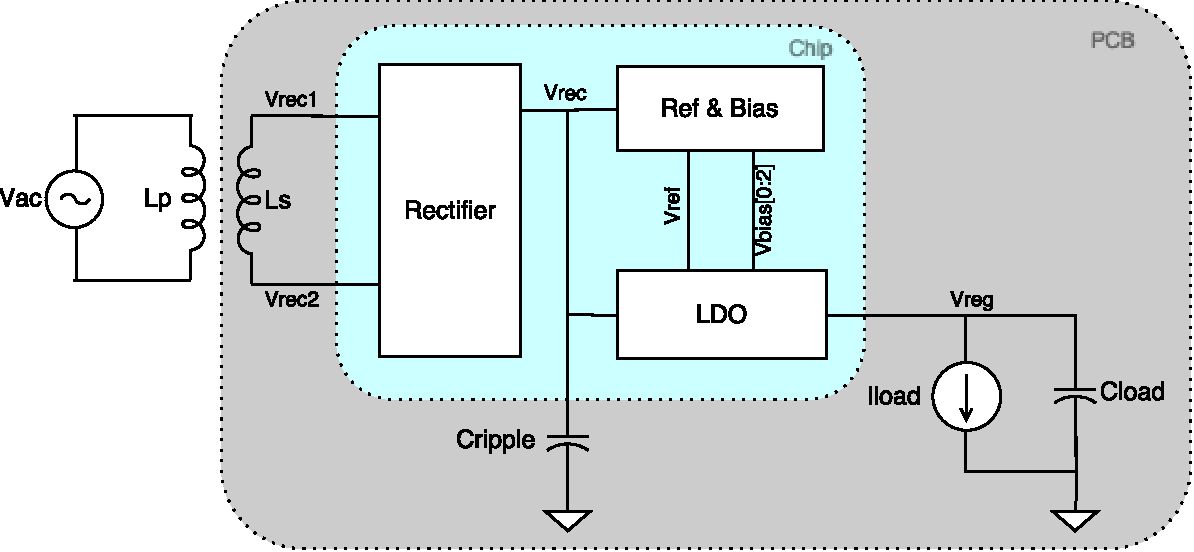
\includegraphics[width=\textwidth]{img/block_diagram.pdf} 
   \caption{Block diagram of complete design}
   \label{fig:blockd}
\end{figure}

As shown in the block diagram above, the design includes inductors, rectifier, LDO and reference and biasing circuits. The following is the design discussion of each sub circuits.

\section{Rectifier}

\cite{rectcomp} has discussed different CMOS implementations of rectifier topologies in terms of tradeoffs and performance comparisons. 
Basically, there are two different approach of implementing rectifer in CMOS: active and passive.
The most basic rectifier is  the conventional full wave bridge structure where the diodes are replaced by the diode connected MOS devices in CMOS technology. This topology though being simple to implement, it has a major drawback. It requires at least twice the threshold of a MOS device as there are two diode connected MOSes in the conduction path and this limits its use in the devices powered by low voltages. 

In order to overcome the problem of large voltage drop in the conventional rectifier, two popular techniques are implemented: passive and active. In passive rectifier, threshold voltage cancellation techniques are used. Whereas in active rectifier, active devices like comparators are used to check if the conduction condition is met and as a result instantly turning on or off ideally.

\newpage
\printbibliography
\end{document}
